\subsection{Experiments}
To show the viability of the framework, three experiments were conducted and the a fixed set of models was tested in these three conditions.
The evaluated models were all combinations of the two representation type (``GridState" and ``VectorState"), the two navigation types (``Optimal" and ``Greedy") and different values of the determinism parameter $\beta$.
Considered values were:

\[
[0,.5,1,2,3,5]
\]

In total, this amounted to 24 model variants.
Both experiments were conducted in a rectangular arena with the dimensions $\{width=20, height=20\}$.
Per experiment, 100 iterations were run, with the true model being chosen randomly from the aforementioned 24 model variants.

\subsubsection{Experiment 1}
For the first experiment, goals and starting point were chosen at random. The only limitation was that the starting point could not be set to the position of any of the goals.
No obstacles were placed in the environment.

\subsubsection{Experiment 2}
For the second experiments, starting position and goals were fixed.
The starting position was always set to the lower left corner $(0,0)$. Goals were placed on symmetric positions in the upper right quarter of the environment.
Goal placement can be seen in Figures \ref{fig:exp2convexobstacles} and Figure \ref{fig:exp2concaveobstacles}.
Two types of obstacles were placed in the environment: convex, and concave.

\paragraph{a) Convex Obstacles}
The convex obstacle can be seen in Figure \ref{fig:exp2convexobstacles}.
Convex obstacles in general are easier to navigate since usually the utility gradient naturally leads around the obstacle.

\begin{figure}
	\centering
	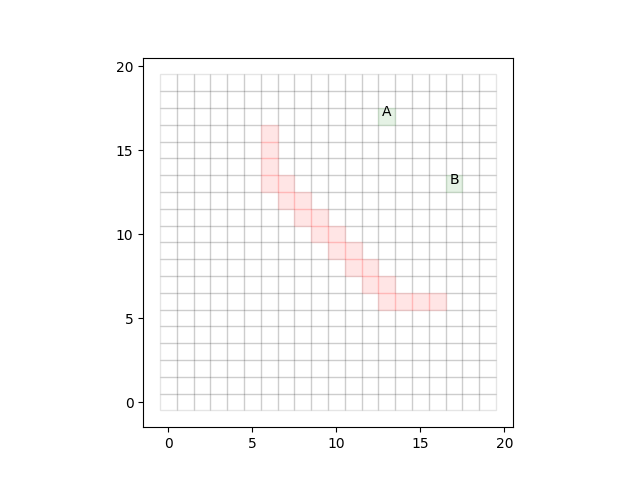
\includegraphics[width=0.8\linewidth]{res/exp2_convex_obstacles}
	\caption{Visualization of Experiment 2a with a convex obstacle between start and goals. Starting position, not depicted in this image, is the lower left corner. Two goals exist in the environment, Goal A and Goal B, whereas Goal A is the true goal and Goal B is the distractor.}
	\label{fig:exp2convexobstacles}
\end{figure}


\paragraph{b) Concave Obstacles.}
The concave obstacle can be seen in Figure \ref{fig:exp2concaveobstacles}.
Concave obstacles present a problem for traditional greedy forms of navigation,
as they introduce a local minimum.
As there were no specific methods implemented to avoid the agent getting caught in local minima, except for the determinism factor, the algorithm was set to end at a maximum of 3000 steps if the goal was not reached.


\begin{figure}
	\centering
	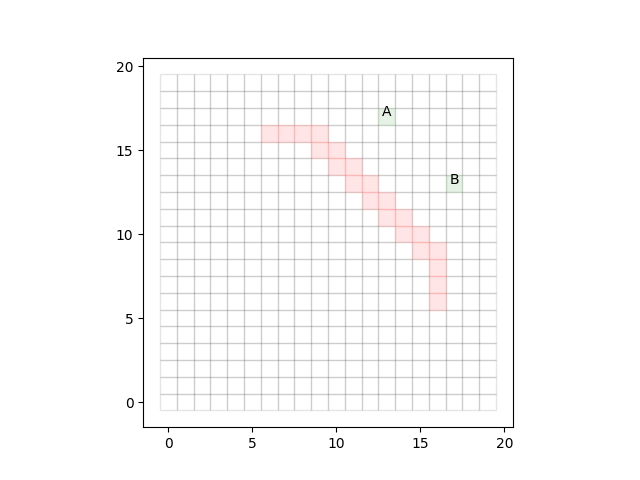
\includegraphics[width=0.8\linewidth]{res/exp2_concave_obstacles}
	\caption{Visualization of Experiment 2b with a concave obstacle between start and goals. Starting position, not depicted in this image, is the lower left corner. Two goals exist in the environment, Goal A and Goal B, whereas Goal A is the true goal and Goal B is the distractor.}
	\label{fig:exp2concaveobstacles}
\end{figure}

